\documentclass[conference]{../cls/IEEEtran}

\usepackage{graphicx}

\begin{document}

\title{Behavior Estimation on Energy-Efficient Urban Traffic Control to Explore
Operational Feasibility}

\author{
	\IEEEauthorblockN{Dominik Ascher}
	\IEEEauthorblockA{
		Chair IV: Software \& Systems Enginesering\\
		Technische Universit\"at M\"unchen\\
		Boltzmannstr.\ 3, 85748 Garching, Germany\\
		Email: ds.ascher@gmail.com
	}
	\and
	\IEEEauthorblockN{Georg Hackenberg}
	\IEEEauthorblockA{
		Chair IV: Software \& Systems Engineering\\
		Technische Universit\"at M\"unchen\\
		Boltzmannstr.\ 3, 85748 Garching, Germany\\
		Email: hackenbe@in.tum.de
	}
}

\maketitle

\begin{abstract}
Many application ideas arise from increasing computational and communicational capabilities of today's automotive vehicles.
Early studies are needed to show the feasability and potential of these ideas to foster future research and development.
\end{abstract}

\begin{IEEEkeywords}
Feasibility study, urban traffic control, eco-routing.
\end{IEEEkeywords}

\section{Motivation}

\textit{State of the art: Urban traffic control (cooperative), agent-based
approaches, congestion management.}

In the recent decades, Urban Traffic Control (UTC) has seen a multitude of
approaches dealing with the complexity of action and interaction between
multiple traffic participants through elaborate control systems
~\cite{Roozemond1999},~\cite{Chen2010}.
In this context, (a large number of) approaches incorporating multi-agent
systems have been developed and have established agent systems as a pervasive
paradigm in traffic simulation and congestion management ~\cite{Chen2010}.

\textit{+Problem: Intersections and Traffic Jams}

\textit{Second direction: Eco-routing (energy efficient, fast, but not
cooperative).}

In this paper, Eco-Routing refers to the concept of selecting the most
energy-efficient route between two locations. 

\textit{+Differing Definitions : ShortestPath + EnergyOptimization Problem
~\cite{Barth2007}}

\textit{+Handling of congestions, most-energy-efficient route possibly
subject to congestion}

 ~\cite{Boriboonsomsin2012} introduced a (reactive) eco-routing (navigation)
 system alleviating the problem of congestion through the
 incorporation of historical and real-time traffic information for individual
 traffic participants.


\textit{Energy-efficient urban traffic control approaches are
missing, i.e.
the combination of urban traffic control and eco-routing.}

In summary, eco-routing approaches offer efficient routing techniques, which
concentrate on the energy-efficient routing of single traffic partipants in
relation to their current environment.  In contrast, UTC approaches utilize the
cooperation and interaction between multiple traffic participants for congestion
management within well-defined boundaries, i.e.
cities. 
However, while the current approaches of both
directions offer feasible techniques/solutions towards specific problems, they are
subject to their limited scope and do not consider an holistic integration of
congestion management with energy-efficient routing (eco-routing). Therefore,
current UTC approaches remain unaligned towards energy-effiency and emission
minimization.

To overcome this situation, in this paper, we report on first steps towards an
operational feasibility study of energy-efficient urban traffic control.
In the following we shortly describe the underlying behavior estimation
framework before explaining the energy-efficient urban traffic control demonstrator as well as initial performance analysis results.

\section{Behavior Estimation Framework}

To illustrate the scope of our work we first give a short definition of feasibility studies: 
According to Whitten et al.~\cite{Whitten2005} in systems engineering feasibility studies follow the requirements discovery phase to uncover potential opportunities and threads.
Upon successful feasibility demonstration the system design, implementation and operation phases follow.

\begin{figure}[b]
	\centering
	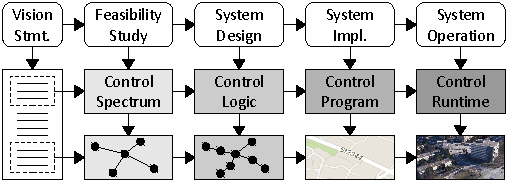
\includegraphics{../gfx/process.pdf}
	\caption{Overview of the general systems engineering process from requirements discovery over feasibility study, system design and implementation to system operation adapted to cooperative eco-routing.}
	\label{figure:process}
\end{figure}
We translate this process to cooperative eco-routing as illustrated in Figure~\ref{figure:process}.
Given the requirements (i.e.\ energy-efficient and congestion-free routing) we develop a control spectrum specification and analyze it with respect to an approximate physical model.
Technically, we base our work on early emergent property estimation techniques described in~\cite{Hackenberg2012}.
Consequently, we use a discrete-time and continuous-state system model as depicted in Figure~\ref{figure:framework}.
We rely on discrete-time models to reduce the reachable state space during analysis.
However, we use continuous-state models because quantities like velocity or distance can be described more intuitively.
Moreover, we rely on a generic and reusable model architecture dividing the system into software, context, constraint, objective and equivalence components.
In particular, the partial software model describes the control spectrum, while the context model describes the physical state.
Based on the physical state the constraint and objective models define the operational limits and goals.
Finally, the equivalence model describes how the physical states can be clustered during state space exploration.
Behavior estimation uses stochastic optimization techniques similar to~\cite{Pereira1991} to approximate optimal system behavior.

\begin{figure}[b]
	\centering
	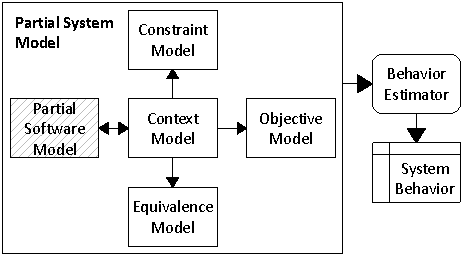
\includegraphics{../gfx/framework.pdf}
	\caption{Overview of the estimation framework including component-based system model (including non-deterministic software component), behavior estimator and system behavior.}
	\label{figure:framework}
\end{figure}

\section{Energy-Efficient Urban Traffic Control}

Model architecture: Context (i.e.\ vehicle) component, constraint component, objective component, control component, equivalence component.

Component behavior: Speed selection, edge selection, edge-based collision detection, energy consumption, etc.

Behavior estimation: One basic case (single vehicle, two routes) and one more complex case (multiple vehicles).

\section{Conclusion and Outlook}

Great stuff! :)


\bibliographystyle{../bst/IEEEtran}
\bibliography{ICCVE-2014}

\end{document}
